\documentclass[a4paper]{article}

\input{style/ch_xelatex.tex}
%\input{style/scala.tex}

%代码段设置
\lstset{numbers=left,
basicstyle=\tiny,
numberstyle=\tiny,
keywordstyle=\color{blue!70},
commentstyle=\color{red!50!green!50!blue!50},
frame=single, rulesepcolor=\color{red!20!green!20!blue!20},
escapeinside=``
}

\graphicspath{ {images/} }
\usepackage{ctex}
\usepackage{graphicx}
\usepackage{color,framed}%文本框
\usepackage{listings}
\usepackage{caption}
\usepackage{amssymb}
\usepackage{enumerate}
\usepackage{xcolor}
\usepackage{bm} 
\usepackage{lastpage}%获得总页数
\usepackage{fancyhdr}
\usepackage{tabularx}  
\usepackage{geometry}
%\usepackage{minted}
\usepackage{graphics}
\usepackage{subfigure}
\usepackage{float}
\usepackage{pdfpages}
\usepackage{pgfplots}
\pgfplotsset{width=10cm,compat=1.9}
\usepackage{multirow}
\usepackage{footnote}
\usepackage{booktabs}

%-----------------------伪代码------------------
\usepackage{algorithm}  
\usepackage{algorithmicx}  
\usepackage{algpseudocode}  
\floatname{algorithm}{Algorithm}  
\renewcommand{\algorithmicrequire}{\textbf{Input:}}  
\renewcommand{\algorithmicensure}{\textbf{Output:}} 
\usepackage{lipsum}  
\makeatletter
\newenvironment{breakablealgorithm}
  {% \begin{breakablealgorithm}
  \begin{center}
     \refstepcounter{algorithm}% New algorithm
     \hrule height.8pt depth0pt \kern2pt% \@fs@pre for \@fs@ruled
     \renewcommand{\caption}[2][\relax]{% Make a new \caption
      {\raggedright\textbf{\ALG@name~\thealgorithm} ##2\par}%
      \ifx\relax##1\relax % #1 is \relax
         \addcontentsline{loa}{algorithm}{\protect\numberline{\thealgorithm}##2}%
      \else % #1 is not \relax
         \addcontentsline{loa}{algorithm}{\protect\numberline{\thealgorithm}##1}%
      \fi
      \kern2pt\hrule\kern2pt
     }
  }{% \end{breakablealgorithm}
     \kern2pt\hrule\relax% \@fs@post for \@fs@ruled
  \end{center}
  }
\makeatother
%------------------------代码-------------------
\usepackage{xcolor} 
\usepackage{listings} 
\lstset{ 
breaklines,%自动换行
basicstyle=\small,
escapeinside=``,
keywordstyle=\color{ blue!70} \bfseries,
commentstyle=\color{red!50!green!50!blue!50},% 
stringstyle=\ttfamily,% 
extendedchars=false,% 
linewidth=\textwidth,% 
numbers=left,% 
numberstyle=\tiny \color{blue!50},% 
frame=trbl% 
rulesepcolor= \color{ red!20!green!20!blue!20} 
}

%-------------------------页面边距--------------
\geometry{a4paper,left=2.3cm,right=2.3cm,top=2.7cm,bottom=2.7cm}
%-------------------------页眉页脚--------------
\usepackage{fancyhdr}
\pagestyle{fancy}
\lhead{\kaishu \leftmark}
% \chead{}
\rhead{\kaishu 并行程序设计实验报告}%加粗\bfseries 
\lfoot{}
\cfoot{\thepage}
\rfoot{}
\renewcommand{\headrulewidth}{0.1pt}  
\renewcommand{\footrulewidth}{0pt}%去掉横线
\newcommand{\HRule}{\rule{\linewidth}{0.5mm}}%标题横线
\newcommand{\HRulegrossa}{\rule{\linewidth}{1.2mm}}
\setlength{\textfloatsep}{10mm}%设置图片的前后间距
%--------------------文档内容--------------------

\begin{document}
\renewcommand{\contentsname}{目\ 录}
\renewcommand{\appendixname}{附录}
\renewcommand{\appendixpagename}{附录}
\renewcommand{\refname}{参考文献} 
\renewcommand{\figurename}{图}
\renewcommand{\tablename}{表}
\renewcommand{\today}{\number\year 年 \number\month 月 \number\day 日}

%-------------------------封面----------------
\begin{titlepage}
    \begin{center}
    \includegraphics[width=0.8\textwidth]{NKU.png}\\[1cm]
    \vspace{20mm}
		\textbf{\huge\textbf{\kaishu{计算机学院}}}\\[0.5cm]
		\textbf{\huge{\kaishu{并行程序设计报告}}}\\[2.3cm]
		\textbf{\Huge\textbf{\kaishu{SIMD加速的高斯消去算法}}}

		\vspace{\fill}
    
    % \textbf{\Large \textbf{并行程序设计期末实验报告}}\\[0.8cm]
    % \HRule \\[0.9cm]
    % \HRule \\[2.0cm]
    \centering
    \textsc{\LARGE \kaishu{姓名\ :\ 王毅豪}}\\[0.5cm]
    \textsc{\LARGE \kaishu{学号\ :\ 2412509}}\\[0.5cm]
    \textsc{\LARGE \kaishu{专业\ :\ 计算机科学与技术}}\\[0.5cm]
    
    \vfill
    {\Large \today}
    \end{center}
\end{titlepage}

\renewcommand {\thefigure}{\thesection{}.\arabic{figure}}%图片按章标号
\renewcommand{\figurename}{图}
\renewcommand{\contentsname}{目录}  
\cfoot{\thepage\ of \pageref{LastPage}}%当前页 of 总页数


% 生成目录
\clearpage
\tableofcontents
\newpage

%--------------------------Title--------------------------------
%--------------------------正文内容开始--------------------------------
\section{实验目标与问题描述}
本次实验的目标是在 ARM 架构平台（华为鲲鹏 920）上，利用 NEON 指令集对普通高斯消去算法进行 SIMD 并行化优化。

高斯消去法是求解线性方程组的核心算法。其核心计算瓶颈在于消去过程中重复进行的浮点乘减运算。通过单指令多数据流（SIMD）技术，我们可以在一个时钟周期内同时处理多个浮点数，从而显著提升算法的执行效率，减少计算延迟。
\section{算法设计与核心代码实现}

\subsection{算法复杂度分析}
普通高斯消去法的空间复杂度主要取决于存储 $N \times N$ 矩阵的二维数组，为 $O(N^2)$。

在时间复杂度方面，串行算法包含三层嵌套循环。最外层循环 $k$ 执行 $N$ 次；中间层 $i$ 执行 $N-k$ 次；最内层 $j$ 进行核心的消去乘减运算，执行 $N-k$ 次。因此，核心消去操作的总执行次数约为：
\begin{equation}
\sum_{k=0}^{N-1} (N-k)^2 \approx \frac{N^3}{3}
\end{equation}
算法的整体时间复杂度为 $O(N^3)$。由于最内层循环的浮点乘减运算占用了绝大部分的执行时间，构成了整个算法的计算热点与性能瓶颈，因此对这部分循环进行 SIMD 向量化改造将获得最大的性能收益。

\subsection{普通高斯消去串行算法}
基于上述分析，串行算法的实现严格遵循三层循环结构。最外层循环 $k$ 遍历矩阵的对角线元素（主元）。对于每个主元，首先进行归一化处理（除法），使得主元变为 1。随后，使用中间层循环 $i$ 遍历主元所在行下方的所有行，利用最内层循环 $j$ 将下方各行的对应元素消为 0（乘减运算）。具体的串行算法核心代码如下：

\begin{lstlisting}[title=普通高斯消去串行算法,frame=trbl,language={C++}]
void gauss_serial(float** A, int n) {
    for (int k = 0; k < n; k++) {
        float vt = A[k][k];
        // 1. 归一化（除法循环）
        for (int j = k + 1; j < n; j++) { 
            A[k][j] = A[k][j] / vt; 
        }
        A[k][k] = 1.0f;
        
        // 2. 消去（乘减循环）
        for (int i = k + 1; i < n; i++) {
            float factor = A[i][k];
            for (int j = k + 1; j < n; j++) { 
                A[i][j] = A[i][j] - factor * A[k][j]; 
            }
            A[i][k] = 0.0f;
        }
    }
}
\end{lstlisting}

\subsection{NEON 向量化加速算法}
在串行算法中，内层的“归一化”和“消去”循环都不存在数据依赖，可以被高度并行化。我们采用 ARM NEON 指令集，通过 128 位向量寄存器（可同时容纳 4 个 32 位单精度浮点数）实现四路数据的并发处理。

\textbf{向量化策略与性能收益探讨（除法 vs. 消去）：}
在算法实现中，高斯消去包含“第 $k$ 行归一化（除法）”和“第 $k$ 行以下消去（乘减）”两个可向量化的部分。
\begin{enumerate}
    \item \textbf{除法部分的向量化：} 位于外层嵌套中，时间复杂度仅为 $O(N^2)$。我们在实现中通过将除法转换为乘以倒数（\texttt{1.0f / vt}），并使用 \texttt{vmulq\_f32} 进行了向量化。虽然这能减少除法的时钟周期，但由于其在整体执行时间中占比较小，对全局加速比的贡献有限。
    \item \textbf{消去部分的向量化：} 位于三重循环最内层，时间复杂度为 $O(N^3)$，是真正的计算热点。我们使用 NEON 融合乘减指令 \texttt{vmlsq\_f32} 对其进行了一次处理 4 个单精度浮点数的向量化。实验数据表明，绝大部分的性能提升（约 2.0x 加速比）均来源于对这部分的向量化改造。这验证了“优化应集中在计算热点（Amdahl 定律）”的并行编程核心原则。
\end{enumerate}

本次向量化优化的核心算法设计策略包括：
\begin{itemize}
    \item \textbf{除法转乘法：} 在归一化步骤中，提前计算好主元的倒数 \texttt{inv\_vt}，将最内层循环的除法操作全部转换为乘法操作，显著减少了 CPU 的时钟周期消耗。
    \item \textbf{向量广播：} 使用 \texttt{vdupq\_n\_f32} 指令将标量数据（主元倒数 \texttt{inv\_vt} 和消去因子 \texttt{factor}）进行广播，填充至整个 128 位向量寄存器的 4 个通道中，为后续的对位运算做准备。
    \item \textbf{并行乘减与非对齐访存：} 考虑到 aarch64 架构对未对齐内存访问有极佳的硬件支持，本实验直接使用 \texttt{vld1q\_f32} 进行未对齐的连续访存，避免了复杂的头部对齐代码。在计算密集的消去循环中，调用了融合乘减指令 \texttt{vmlsq\_f32}，在一个指令周期内同时完成 4 个浮点元素的乘法与减法运算，极大提升了计算吞吐量。
    \item \textbf{循环展开与尾部处理：} 由于高斯消去过程中每次内层循环的起始偏移量 $j$ 不断变化，且矩阵规模无法保证时刻是 4 的倍数。为保证算法正确性，我们将主体循环按步长 4 推进（\texttt{j += 4}），而末尾不足 4 个元素的残余部分（\texttt{j < n}）则退化为标量串行处理。
\end{itemize}

基于以上设计，NEON 向量化版本的完整核心代码实现如下：

\begin{lstlisting}[title=NEON 加速的高斯消去算法,frame=trbl,language={C++}]
#include <arm_neon.h>

void gauss_neon(float** A, int n) {
    for (int k = 0; k < n; k++) {
        float vt = A[k][k];
        float inv_vt = 1.0f / vt;
        float32x4_t inv_vt_vec = vdupq_n_f32(inv_vt); 
        int j = k + 1;
        
        // 1. 归一化循环的向量化
        for (; j <= n - 4; j += 4) {
            float32x4_t a_kj = vld1q_f32(&A[k][j]); 
            float32x4_t res = vmulq_f32(a_kj, inv_vt_vec); 
            vst1q_f32(&A[k][j], res); 
        }
        // 归一化尾部标量处理
        for (; j < n; j++) { A[k][j] = A[k][j] * inv_vt; }
        A[k][k] = 1.0f;
        
        // 2. 消去循环的向量化
        for (int i = k + 1; i < n; i++) {
            float factor = A[i][k];
            float32x4_t factor_vec = vdupq_n_f32(factor); 
            j = k + 1;
            for (; j <= n - 4; j += 4) {
                float32x4_t a_ij = vld1q_f32(&A[i][j]); 
                float32x4_t a_kj = vld1q_f32(&A[k][j]); 
                // 调用 NEON 融合乘减运算
                float32x4_t res = vmlsq_f32(a_ij, a_kj, factor_vec); 
                vst1q_f32(&A[i][j], res); 
            }
            // 消去尾部标量处理
            for (; j < n; j++) { A[i][j] = A[i][j] - factor * A[k][j]; }
            A[i][k] = 0.0f;
        }
    }
}
\end{lstlisting}

\section{实验环境}
本次实验的硬件平台与软件栈均基于南开大学提供的高性能计算集群，具体环境配置如下：

\begin{itemize}
    \item \textbf{硬件平台：} 华为鲲鹏 920 处理器，基于 ARM AArch64 架构。
    \item \textbf{操作系统：} openEuler 操作系统。
    \item \textbf{编译器：} GCC (g++)，编译时统一开启 \texttt{-O2} 级别的优化。
    \item \textbf{任务调度系统：} 由于集群的主节点（Master Node）严禁直接运行高负载的可执行文件，本次实验的程序运行均通过 PBS 任务调度系统（使用 \texttt{qsub} 命令）提交至计算节点执行。
\end{itemize}

\section{实验过程}
参考普通高斯消去算法的特点，本次实验在 ARM 平台上的完整测试验证过程分为以下几个阶段：

\subsection{代码编译与运行提交}
由于集群的计算节点通过作业调度系统管理，我们无法像在本地机器上那样直接运行可执行文件。首先，在主节点的终端中使用 \texttt{g++} 进行编译，并显式指定 \texttt{-O2} 优化选项：
\begin{lstlisting}[language=bash, frame=single, numbers=none]
$ g++ -O2 main.cc -o main
\end{lstlisting}

编译成功并生成 \texttt{main} 可执行文件后，使用实验框架提供的测试脚本提交作业。脚本内部封装了 \texttt{qsub} 命令，将任务投递至计算节点：
\begin{lstlisting}[language=bash, frame=single, numbers=none]
$ sh test.sh 1 1
\end{lstlisting}

\subsection{作业监控与数据提取}
任务提交后，通过 \texttt{qstat} 命令实时监控作业的排队与执行状态。当对应作业 ID 的状态栏（S列）变为 \texttt{C}（Completed）时，说明计算节点已完成高斯消去算法的执行。

程序的标准输出与标准错误会被重定向到当前目录下的日志文件中（如 \texttt{test.o} 或 \texttt{.o} 后缀的文件）。使用 \texttt{ls -lt} 按时间排序找到最新生成的日志文件，并使用 \texttt{cat} 命令读取内容以提取耗时数据：
\begin{lstlisting}[language=bash, frame=single, numbers=none]
$ cat test.o
Matrix Size : 1024x1024
Serial Latency : 426.937 (ms) 
NEON Latency   : 207.863 (ms) 
Speedup        : 2.05394x
\end{lstlisting}
通过不断修改源文件中的矩阵规模常量 $N$，重复上述“编译-提交-读取日志”的流程，我们分别收集了 $N=512, 1024, 2048$ 三组规模下的串行与 NEON 并行性能数据。

\subsection{反汇编代码导出}
为了细致分析程序性能表现的内在原因，验证 NEON 向量化指令是否被编译器正确生成，我们在主节点上使用 \texttt{objdump} 工具对编译得到的二进制文件进行了反汇编，将 ARM64 汇编指令导出至本地文本文件中以供静态分析：
\begin{lstlisting}[language=bash, frame=single, numbers=none]
$ objdump -d main > asm.txt
\end{lstlisting}
通过搜索 \texttt{gauss\_neon} 与 \texttt{gauss\_serial} 的函数符号，我们提取了核心计算循环的汇编代码片段，这为后续的性能内在原因分析提供了硬核的底层数据支撑。
\section{实验结果与性能表现分析}

\subsection{性能测试结果}
本节展示了在华为鲲鹏 920 处理器（ARM AArch64 架构）上，矩阵规模 $N$ 分别为 512、1024、2048 时，普通高斯消去算法的串行版本与 NEON 向量化版本的性能差异。程序编译优化选项统一为 \texttt{-O2}。详细的耗时与加速比数据如表 \ref{table:results} 所示。

\begin{table}[H]
  \centering
  \begin{tabular}{|c|c|c|c|}
  \hline
  矩阵规模 ($N$) & 串行耗时 (ms) & NEON 向量化耗时 (ms) & 加速比 \\
  \hline
  $512 \times 512$ & 47.0312 & 22.4076 & 2.09889x \\
  \hline
  $1024 \times 1024$ & 426.937 & 207.863 & 2.05394x \\
  \hline
  $2048 \times 2048$ & 3575.58 & 1730.09 & 2.06670x \\
  \hline
  \end{tabular}
  \caption{不同规模下高斯消去算法的性能对比（串行 vs NEON）}
  \label{table:results}
\end{table}

为了更直观地展示性能随问题规模的变化趋势，我们将上述数据分别绘制为执行时间与加速比的折线对比图。

\begin{figure}[H]
    \centering
    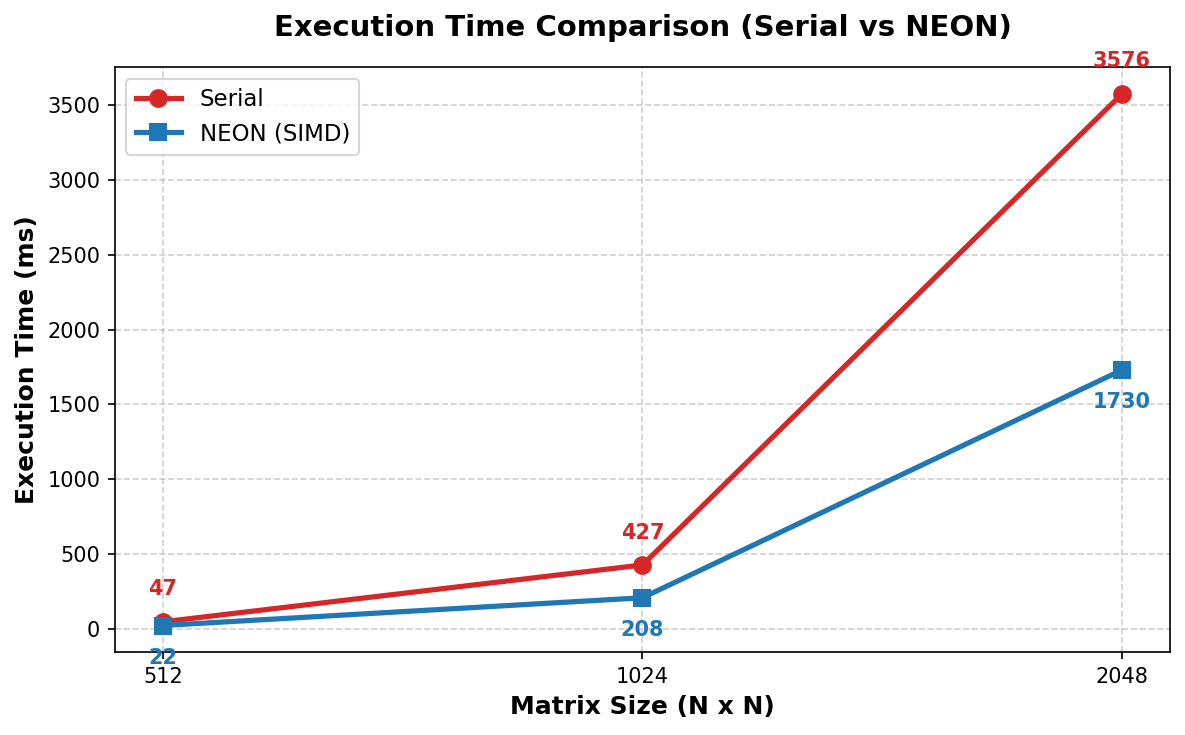
\includegraphics[width=0.8\textwidth]{p2.pdf}
    \caption{不同矩阵规模下的执行时间对比。随着 $N$ 的成倍增加，串行算法和 NEON 并行算法的执行时间均呈现出符合 $O(N^3)$ 复杂度的陡峭非线性增长，但 NEON 版本始终保持显著的时间削减。}
    \label{fig:exec_time}
\end{figure}

\begin{figure}[H]
    \centering
    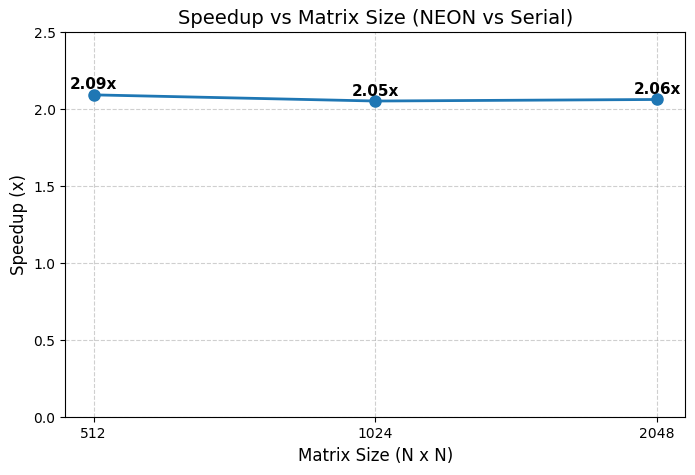
\includegraphics[width=0.8\textwidth]{p1.pdf}
    \caption{不同矩阵规模下 NEON 向量化算法的加速比。在 $N \ge 512$ 的较大规模区间内，加速比曲线表现得非常平缓，稳定在 2.05x 至 2.09x 之间。}
    \label{fig:speedup}
\end{figure}

\subsection{性能表现的内在原因分析}
参考计算机体系结构相关原理，我们结合底层汇编代码对上述实验现象及其背后的内在性能瓶颈进行深入剖析。

\subsubsection{汇编指令级并行与 FMA 优化}
NEON 向量化版本能够取得超过 2.0x 稳定加速比的核心原因，在于底层指令级的极致优化。通过 \texttt{objdump} 工具反编译生成的可执行文件，我们观察到：
\begin{itemize}
    \item \textbf{访存带宽的提升：} 串行版本在最内层循环中频繁使用标量加载指令（如 \texttt{ldr s}），而 NEON 版本使用了 \texttt{ldr q} 系列指令（128 位向量寄存器加载）。CPU 仅用一条指令即可从内存中连续抓取 4 个单精度浮点数，数据加载效率达到了原本的 4 倍。
    \item \textbf{融合乘减（FMA）指令的调用：} 在最内层的核心消去循环中，NEON 汇编代码成功调用了 \texttt{fmls}（Fused Multiply-Subtract）指令。该指令能够在一个时钟周期内合并完成乘法和减法，并且一次性并行处理 4 路数据，大幅压缩了指令发射总数和执行周期。
\end{itemize}

\subsubsection{数据对齐及 Cache 瓶颈分析}
如图 \ref{fig:speedup} 所示，当矩阵规模从 1024 增加到 2048 时，加速比并未随计算密度的增加而继续呈线性上升，而是表现出在 2.0x 上下平稳波动的特征。这一现象反映了底层硬件架构对算法性能的制约：
\begin{itemize}
    \item \textbf{计算密集向访存密集的转移：} 当矩阵规模达到 $2048 \times 2048$ 时，仅存储单精度浮点矩阵就需要 16MB 的内存空间。这一数据量已经远远超出了鲲鹏 920 处理器 L1 和 L2 Cache 的容量限制。此时，算法的性能瓶颈从 CPU 的“计算限制（Compute-bound）”逐渐转移到了“内存带宽限制（Memory-bound）”。Cache Miss 率的急剧上升导致 NEON 的高效计算单元不得不频繁处于等待内存数据搬运的停顿状态。
    \item \textbf{非对齐访存与额外开销的权衡：} 本次实验中，我们在 NEON 算法设计上直接使用了支持非对齐访存的 \texttt{vld1q\_f32} 指令，而未在二维数组分配时进行严格的 Cache Line 对齐（Padding）。虽然不对齐加载策略避免了编写复杂的边界判断逻辑，使得指令流水线更加顺畅，但在 $N=2048$ 这种极端大规模数据下，跨 Cache Line 加载带来的轻微访存惩罚也在一定程度上限制了并行加速比向理论上限的进一步突破。
\end{itemize}

%--------------------------正文内容结束--------------------------------
\newpage
% 附录：Git 项目链接 
\section*{附录：Git 项目链接}
本实验的完整源代码及提交记录已托管至 Git 平台，项目仓库地址如下：\\
\url{https://github.com/NKU025/SIMD-Gaussian-Elimination.git} % 请将这里替换为你自己的实际链接

% 参考文献部分
\renewcommand{\refname}{参考文献}
\begin{thebibliography}{99}

\bibitem{quinn} 
Michael J. Quinn. 
\textit{Parallel Programming in C with MPI and OpenMP} [M]. 
McGraw-Hill Education, 1994.

\bibitem{golub} 
Gene H. Golub and Charles F. Van Loan. 
\textit{Matrix Computations} [M]. 
Johns Hopkins University Press, 2014.

\bibitem{joseph} 
J. Joseph. 
\textit{Parallel Programming: Concepts and Practice} [M]. 
Cambridge University Press, 2022.

\bibitem{arm_neon} 
ARM Developer. 
\textit{Neon Intrinsics Reference} [EB/OL]. 
\url{https://developer.arm.com/architectures/instruction-sets/intrinsics/}

\end{thebibliography}
\end{document}